% !TEX root =  master.tex
\chapter{Analyse} \label{analyse}
	
	Analyse für den Durchblick.
	Studium, Modul \enquote{Fallstudie} et cetera
	
	\section{Anforderungsanalyse}
	
	\section{Ist-Analyse}
	Mithilfe der Ist-Analyse wird eine bestehende Lösung zur Reservierung von Kinokarten betrachtet und evaluiert. Diese Betrachtung bildet die Grundlage für die Evaluierung der verschiedener Aufbauten der Kinoreservierungssysteme. Dabei spielen vor allem die Verständlichkeit der Seite und die verschiedenen Schritte, die für eine Reservierung nötig sind eine entscheidende Rolle. Außerdem wird verglichen, welche Schritte für die Reservierung notwendig sind, mit den verschiedenen Seiten, auf die man weitergeleitet wird. Dabei wird versucht herauszufinden, welche Funktionen für eine Reservierung essenziell sind und welche zusätzliche Funktionen darstellen. Des Weiteren werden die verschiedenen Möglichkeiten einer Bestätigung betrachtet, sowie die Notwendigkeit eines Benutzerkontos. 
	
	\subsection{Kinopolis Viernheim}
	Beim Öffnen der Seite fällt auf, dass das Hauptfenster zur Reservierung von Karten von einem Rahmen mit Werbung für einen aktuellen Film umgeben ist (siehe Abb. \vref{fig:Kinop.Start}). Nach dem Klicken auf diesen Teil der Seite, wird der Nutzer zu einer Übersichtsseite dieses Films weitergeleitet. 
	\begin{figure}
		\centering 
		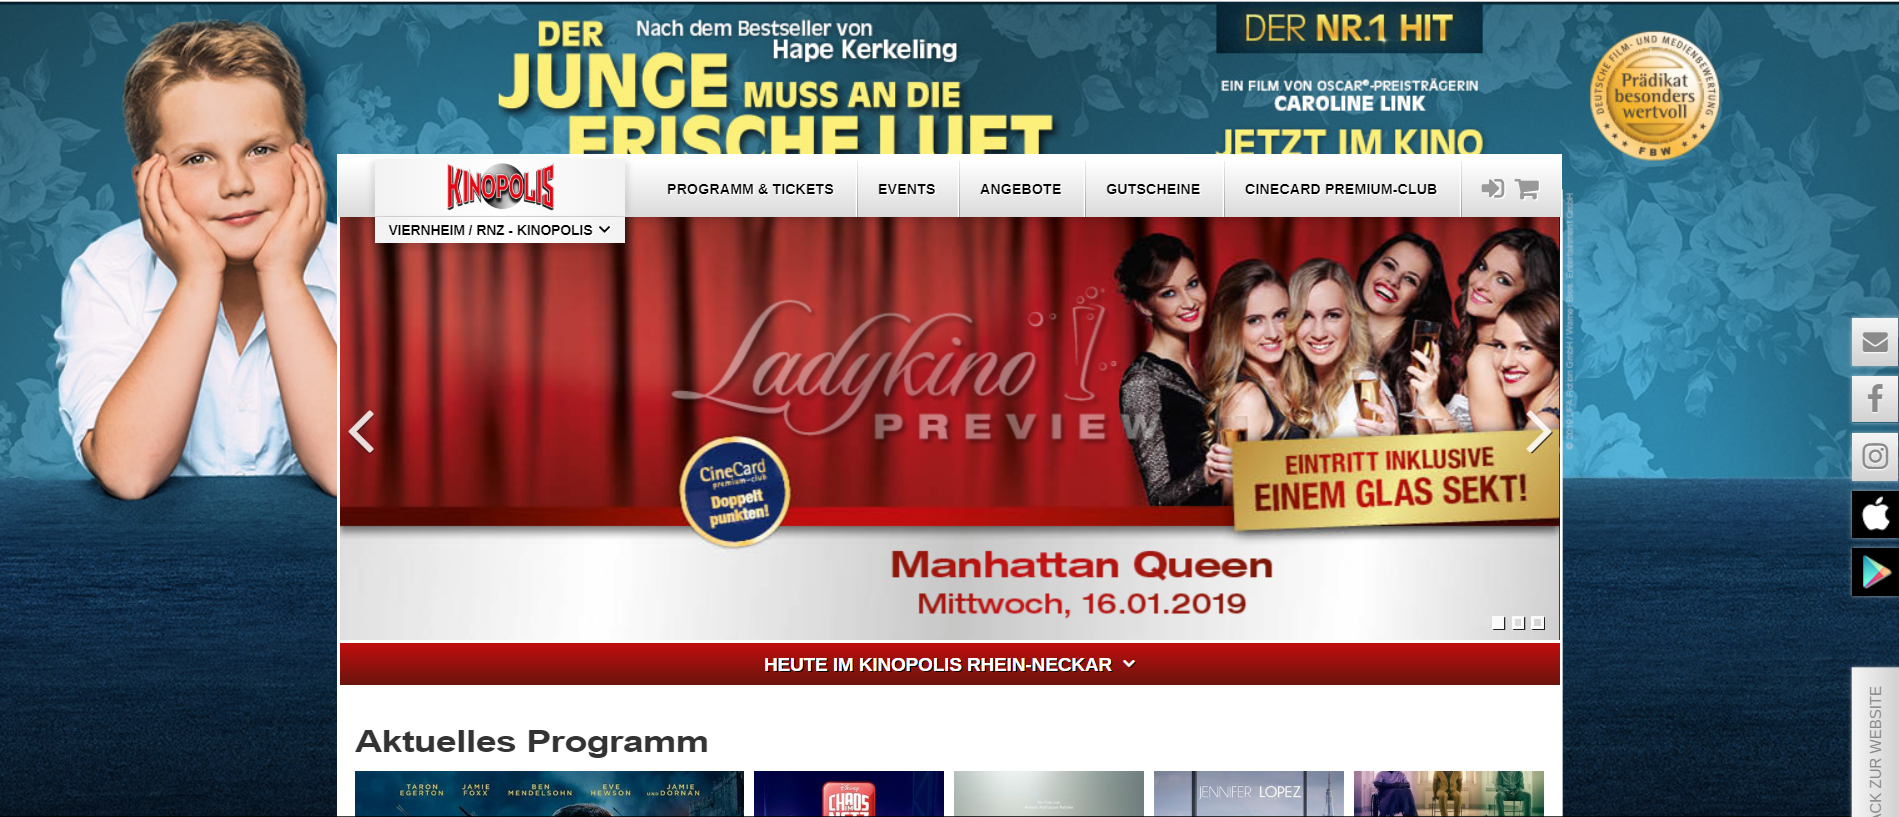
\includegraphics[scale=0.38]{img/Kinopolis_MA_Startseite.png}
		\captionsetup{format=hang}
		\centering\caption[Startseite von Kinopolis Viernheim]{\label{fig:Kinop.Start}Startseite von Kinopolis\footnotemark}
	\end{figure} \footnotetext{Quelle: https://www.kinopolis.de/vi}
	\\Die eigentliche Hauptseite in der Mitte enthält eine Kopfleiste, in der zwischen Programm \& Tickets sowie zwischen Events, Angeboten und Gutscheinen gewählt werden kann. Außerdem besteht die Möglichkeit, sich für eine Premium-Club Card zu registrieren, um Punkte sammeln und diese in Vorteile umwandeln zu können. Des Weiteren ist über ein Symbol die Anmeldung zu einem eingerichteten Account möglich. Unterhalb des Kopfs informiert eine Leiste mit wechselndem Inhalt über Events zu aktuellen Filmen. Als Beispiel wird unter anderem eine \enquote{Ladykino Preview} und ein sich bewegender Sitz angepriesen. 
	\\Nachfolgend findet der Nutzer unter der Überschrift \enquote{Aktuelles Programm} einige ausgewählte Filme. Sie werden in der Plakatansicht dargestellt (siehe Abb. \vref{fig:Kinop.Start2}), weshalb für den Nutzer auf den ersten Blick nur das Filmplakat und der Titel ersichtlich sind. Mithilfe des darunterliegenden Buttons können weitere aktuelle Filme angezeigt werden. Durch das Führen der Maus auf das Plakat eines Films, ergibt sich die Auswahl zwischen dem Anschauen des Trailers, dem Lesen von Filminformationen und dem direkten Kauf von Tickets über die Auswahl der Vorstellung.
	\begin{figure}
		\centering 
		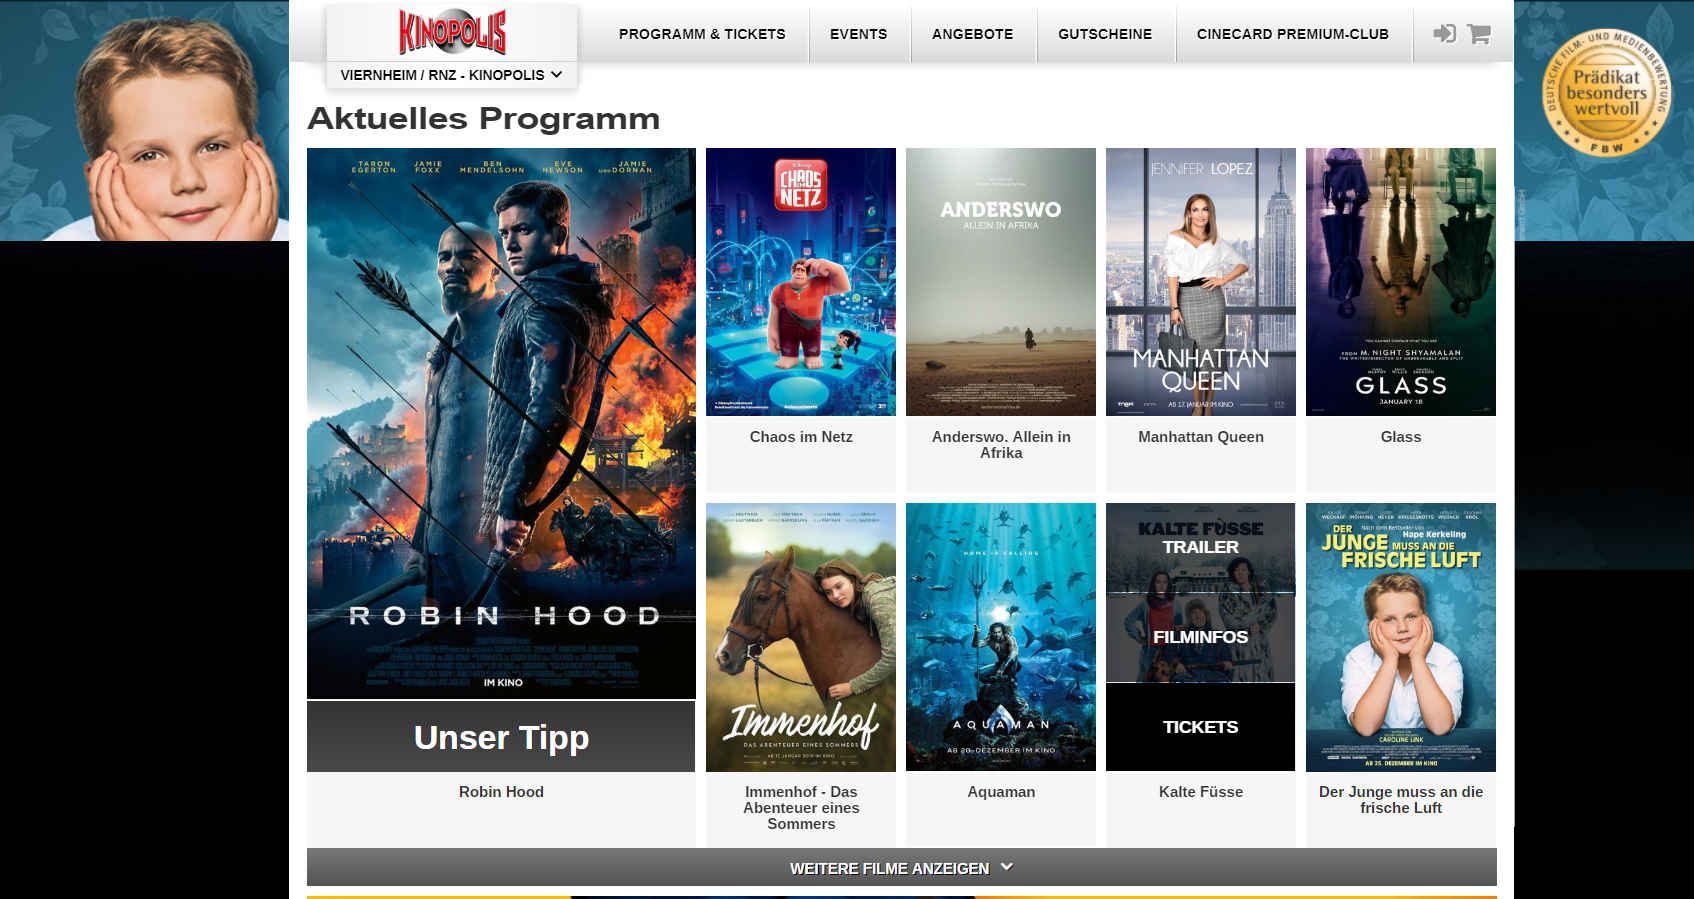
\includegraphics[scale=0.38]{img/Kinopolis_MA_Start2.png}
		\captionsetup{format=hang}
		\centering\caption[Startseite von Kinopolis Viernheim]{\label{fig:Kinop.Start2}Startseite von Kinopolis\footnotemark}
	\end{figure}
	\footnotetext{Quelle: https://www.kinopolis.de/vi}
	Neben diesen Bereichen enthält die Startseite von Kinopolis ebenfalls Informationen zu aktuellen Events, wie \enquote{Kids Previews} und \enquote{Ladykino}. Darüber hinaus bieten sich darunter befindende Abschnitte Auskunft zu Filmen, die bald anlaufen werden, sowie Nachrichten aus Hollywood. 
	
	Die zweite Möglichkeit zur Auswahl eines Filmes besteht durch den zweiten Tab \enquote{Programm \& Tickets}. Dort befindet sich zunächst eine Leiste, in der die Vorstellungen für einen bestimmten Tag oder für eine ganze Woche angezeigt werden können. Standardmäßig ist die Übersicht einer Woche ausgewählt (siehe Abb.\vref{fig:Kinop.Progr.}), wodurch zu jedem Film alle Vorstellungen der Woche aufgelistet sind. Neben der zeitlichen Eingrenzung der Suche, können mit dem in der Abbildung ausgeklappten Programmfilter weitere Eingrenzungen erfolgen. Die Filterung kann nach Genre, FSK-Stufen, Art der Darstellung (2D, 3D,...) und nach zeitlicher Eingrenzung eines Tages erfolgen. Durch die zuletzt genannte Filtermöglichkeit, wird der Beginn der Vorstellungen in Vormittags, Nachmittags und Abends eingestuft.
	\\Rechts neben dem Programmfilter kann je nach Präferenz des Nutzers zwischen zwei Ansichten für die Auflistung der Filme gewechselt werden. Zur Auswahl steht die Listenansicht, sowie die Plakatansicht. Voreingestellt ist die Listenansicht, in der die Filme untereinander dargestellt werden. Zu jedem Film sind Eckdaten wie beispielsweise das Genre, die Länge, und der Start (die erste Vorstellung dieses Films) angegeben. Außerdem wird durch Labels unterstützend ersichtlich, welche FSK-Stufe für den Film besteht. Zusätzliche Labels unterrichten den Nutzer über spezielle Events sowie Angebote. Des Weiteren wird ein Überblick über die Vorstellungen eines Films der kommenden Woche geboten. Dabei wird neben der Zeit ebenfalls der Saal angegeben. Durch das Überfahren einer Vorstellung mit der Maus bekommt der Nutzer die Eckdaten des jeweiligen Saals angezeigt. Bei speziellen Anforderungen an den Saal, kann der Nutzer über den Button \enquote{Saalübersicht} die Daten zu allen vorhandenen Sälen abrufen und somit viel Zeit bei der Suche nach einem Kinosaal, der die Anforderungen erfüllt, sparen. Im nächsten Schritt kann der Nutzer entweder weitere Informationen zu einem Film anschauen, indem er auf den Button \enquote{Filminfos} oder auf den Titel klickt. Dadurch wird der Nutzer auf eine Detailseite weitergeleitet, die im nachfolgend erläutert wird. Wenn der Nutzer bereits eine Vorstellung ausgewählt hat, bekommt er durch das Anklicken der Vorstellung auf die Reservierungsseite weitergeleitet. 
	\\Die Plakatansicht als zweite Möglichkeit der Darstellung ist ähnlich aufgebaut, wie die Darstellung der Filme auf der Startseite. Der Nutzer sieht die verschiedenen Filmplakate und den Titel dieser. Es liegt also an dem Nutzer, ob er zusätzliche Informationen zu dem Film direkt ersichtlich haben möchte oder nicht.  
	\\Neben den zwei erklärten Seiten, bietet das Portal weitere Seiten mit Informationen über Events, Angebote und anderen Vorteilen, die nicht zwingend zur Reservierung von Karten notwendig sind. Deshalb werden diese Seiten in der Ist-Analyse zwar registriert, aber nicht als essenzielle Anforderungen an ein Kinoreservierungssystem erfasst. Aus diesem Grund werden sie nicht näher erläutert.
	\begin{figure}
		\centering 
		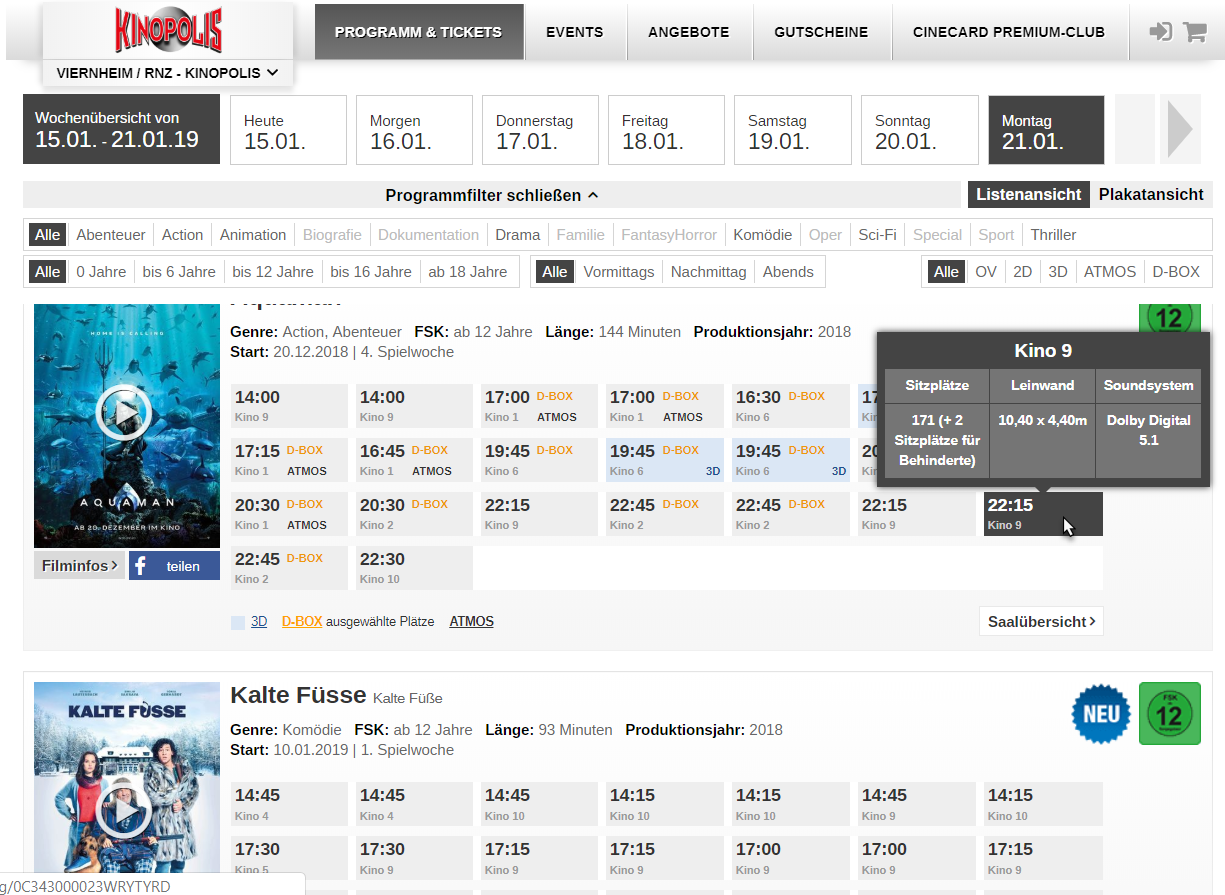
\includegraphics[scale=0.45]{img/Kinopolis_Programm_Tickets.png}
		\captionsetup{format=hang}
		\centering\caption[Startseite von Kinopolis Viernheim]{\label{fig:Kinop.Progr.}Programm \& Tickets von Kinopolis\footnotemark}
	\end{figure}
	\footnotetext{Quelle: https://www.kinopolis.de/vi}
	
	Eine weitere Unterstützung zur Auswahl eines Kinofilms bietet die Detailseite, die einen Überblick über Trailer, die wichtigsten Informationen und die verschiedenen Vorstellungen bietet. Der Nutzer kann die  Detailseite erreichen, indem er auf der Startseite, nach Positionierung der Maus über dem gewünschten Filmplakat, auf die Option Filminfos klickt. Ein solcher Button befindet sich auch in der Seite Programm \& Tickets unterhalb des Trailers. Zusätzlich dazu kann auch der Nutzer über den Filmtitel auf die Detailseite navigieren. 
	\\Dort werden zunächst verschiedene Videos zur Auswahl gestellt. Darunter befindet sich der Trailer und je nach Film weitere Videos, wie beispielsweise das Making-Of. Des Weiteren kann der Nutzer das Filmplakat und eine Bewertung nach 5-Sterne-System sehen und auch selbst abgeben. Über die Eckdaten des Films gelangt der Nutzer in einen Bereich, indem der Inhalt des Film geschildert wird. Dieser ist in deutsch, sowie in einem anderen Tab auch in englisch vorhanden. Ein dritter Tab führt zu Bildern von verschiedenen Szenen des Films. Der darunterliegenden Bereich zeigt eine Übersicht der Vorstellungen für die nächsten sieben Tage. Jede Vorstellung enthält die Startzeit, den Saal, sowie das Vorhanden sein von speziellen Sitzen und ob der Film in 3D läuft. Als Nächstes wird die Besetzung des Films aufgeführt. Dazu werden die wichtigsten Schauspieler des Films mit ihren Namen und einem Foto gezeigt.  
	
	Wenn sich der Nutzer für eine bestimmte Vorstellung entschieden hat, gelangt er durch das Anklicken dieser Vorstellung zur Reservierungsseite. Die Auswahl der Vorstellung kann in der zuletzt vorgestellten Detailseite über die angezeigten Vorstellungen der nächsten Woche, sowie über die Seite \enquote{Programm \& Filme} und die Startseite durch das Anklicken von \enquote{Tickets} erfolgen. 
	\\Die nachfolgende Seite enthält die Möglichkeit der Platzauswahl in dem jeweiligen Kinosaal der Vorstellung. Es wird nochmals das Filmplakat gezeigt, wodurch sich der Nutzer sich sein kann, die Karten für den gewünschten Film auszuwählen. Zusätzlich wird das Datum und die Uhrzeit der Vorstellung angegeben, wodurch eine Verwechslung ausgeschlossen ist.
	Nachfolgend kann der Nutzer entscheiden ob er die Karten kaufen oder reservieren möchte, mit dem Unterschied, dass bei einem Kauf der Karten ermäßigte Tickets für Kinder, Schüler, Studenten und Senioren gekauft werden können. Bei einer Reservierung wird nur die Anzahl der Karten ausgewählt und eventuelle Ermäßigungen müssen an der Kasse besprochen werden. Außerdem muss bei verschiedenen Preiskategorien der Plätze neben dem Wählen der Anzahl auch die Kategorie der Sitzplätze gewählt werden, damit nachfolgend nur Plätze der gewünschten Kategorie gewählt werden können. 
	Wenn der Nutzer eine bestimmte Anzahl ausgewählt hat, kann er mithilfe eines visualisierten Sitzplans seine bevorzugten Plätze wählen. Die Abbildung enthält die Position der Leinwand, den Eingang und die Treppen des Saals. Jeder Sitz des Raums ist eingezeichnet und enthält durch seine Darstellung Informationen über den Buchungsstatus. Durch die farblich verschiedenen Plätze kann der Nutzer die Preiskategorien voneinander unterscheiden, sowie auf einen Blick erkennen, welche Plätze bereits belegt und welche Plätze nicht buchbar sind. 
	\\Hat sich der Nutzer für bestimmte Plätze entschieden, so kann er diese in der Platzkarte auswählen. In diesem Reservierungssystem können nur Plätze nebeneinander gebucht werden, wodurch die Anzahl der ausgewählten Plätze immer nebeneinander liegt. Dadurch wird versucht einzelne buchbare Sitze zwischen gebuchten Sitzen zu vermeiden. Nach der Platzwahl kann ein Nutzer die Karten kaufen bzw. reservieren. 
	
	Dazu gelangt er über einen erscheinenden Button zunächst auf eine Seite, die einen Überblick über die gewählten Produkte gibt. Der Nutzer kann sich entscheiden, ob er die Karten mit vorhandenem Kundenkonto über einen Login oder als Gast kaufen bzw. reservieren möchte. Außerdem besteht die Möglichkeit ein neues Nutzerkonto anzulegen. Bei der Wahl des Gastzugangs wird der Nutzer aufgefordert seinen Namen, sowie E-Mail und Geburtsdatum anzugeben. 
	Beim Reservieren von Karten können die Karten durch den Button \enquote{Jetzt reservieren} reserviert werden, wodurch der Nutzer eine Reservierungsnummer als Bestätigung zugewiesen bekommt. Mit dieser kann er die Karten bis eine halbe Stunde vor Beginn der Vorstellung an der Kasse abholen. Auf der Bestätigungsseite bekommt der Nutzer ebenfalls die Möglichkeit die Reservierung zu drucken, sodass er sie auch ausdrucken könnte. Des Weiteren hat der Kunde die Möglichkeit die Karten zu kaufen oder direkt zu stornieren. 
	\\In dem Kaufvorgang gelangt der Kunde nach dem Anklicken von \enquote{Weiter} in die Ansicht des Warenkorbs, welche die wichtigsten Informationen zu der Vorstellung und dem Standort des Kinos enthält. Außerdem werden Reihe und Plätze der Sitze mit ihrem dazugehörigen Preis angezeigt. Danach muss die Zahlungsmethode gewählt werden, wobei die verschiedenen Auswahlmöglichkeiten zunächst schwer zu erkennen sind. Nach der Auswahl werden die Tickets bezahlt und der Kunde kann in dem Kino direkt reingehen ohne sich zuvor an der Kasse anstellen zu müssen. 
	
	\textbf{Bilder von Detailsseite?; von Auswahl der Sitze; Reservierungsansicht}
	\textbf{Text dazuschreiben, warum nur die Bilder der Reservierung genommen werden?}
	
	\subsubsection{Zusammenfassung der erforderlichen Schritte} 
	Für eine Reservierung von Karten sind vier Schritte von Bedeutung. Zunächst muss sich der Nutzer für einen Film entscheiden. Dies kann durch den Trailer oder das Lesen der Filmbeschreibung geschehen. Nachfolgend wählt der Kunde einen Tag und eine Uhrzeit aus, an dem er sich den Film anschauen möchte. In dem nächsten Schritt entscheidet er sich für eine bestimmte Anzahl an Plätzen sowie wo sich die Sitze in dem Kinosaal befinden sollen. Als letzter Schritt erfolgt die Reservierung der Tickets indem der Kunde seine Daten angibt und dadurch eine Reservierungsnummer mitgeteilt bekommt, mit der er die Karten im Kino abholen kann.
	
	\section{Soll-Analyse}
		
	 	\subsection{User-Research-Prozess} 
	 	User Research ist eine systematische Untersuchung der Ziele, Bedürfnisse und Fähigkeiten der Benutzer\autocite[Vgl.][S. 6]{Schumacher.2010}.
	 	Durch diesen Prozess lässt sich sicherstellen, dass die entwickelte Software den Nutzern einen Mehrwert bietet und an deren Bedürfnisse angepasst ist.
		Der Prozess startet mit der Definition der \textit{User Profile}. Diese klassifizieren Endanwender mit Nutzerprofilen, damit eine konkrete Vorstellung der Anwender geschaffen wird. Anhand von detaillierten Beschreibungen von Attributen lässt sich die Nutzergruppe identifizieren.
		
		\begin{table}[H]
			\centering
			\begin{tabular}{p{5,5cm} || c | c }
				\textbf{Attribute} & \textbf{Endanwender} & \textbf{Mitarbeiter} \\\toprule
				Alter &  16 - 99 Jahre &  16 - 99 Jahre \\
				Geschlecht &  männlich und weiblich &  männlich und weiblich  \\
				Medienkompetenz &  ja und nein &  ja  \\
				Erfahrung Onlinereservierung &  ja und nein &  ja  \\
			\end{tabular}
			\caption[User Profile]{\label{tab:tabelleUserProfile}User Profile}
		\end{table}
		
		Im nächsten Schritt werden Personas aus den User Profiles erstellt. Personas sind fiktive Personen, die für eine Nutzergruppe steht. Der Zweck von Personas ist, dass Entwickler Empathie und Einfühlungsvermögen zu den konkreten Anwendern aufbauen können. 
		
		\begin{figure}[H]
			\subfigure[Persona Franzi]{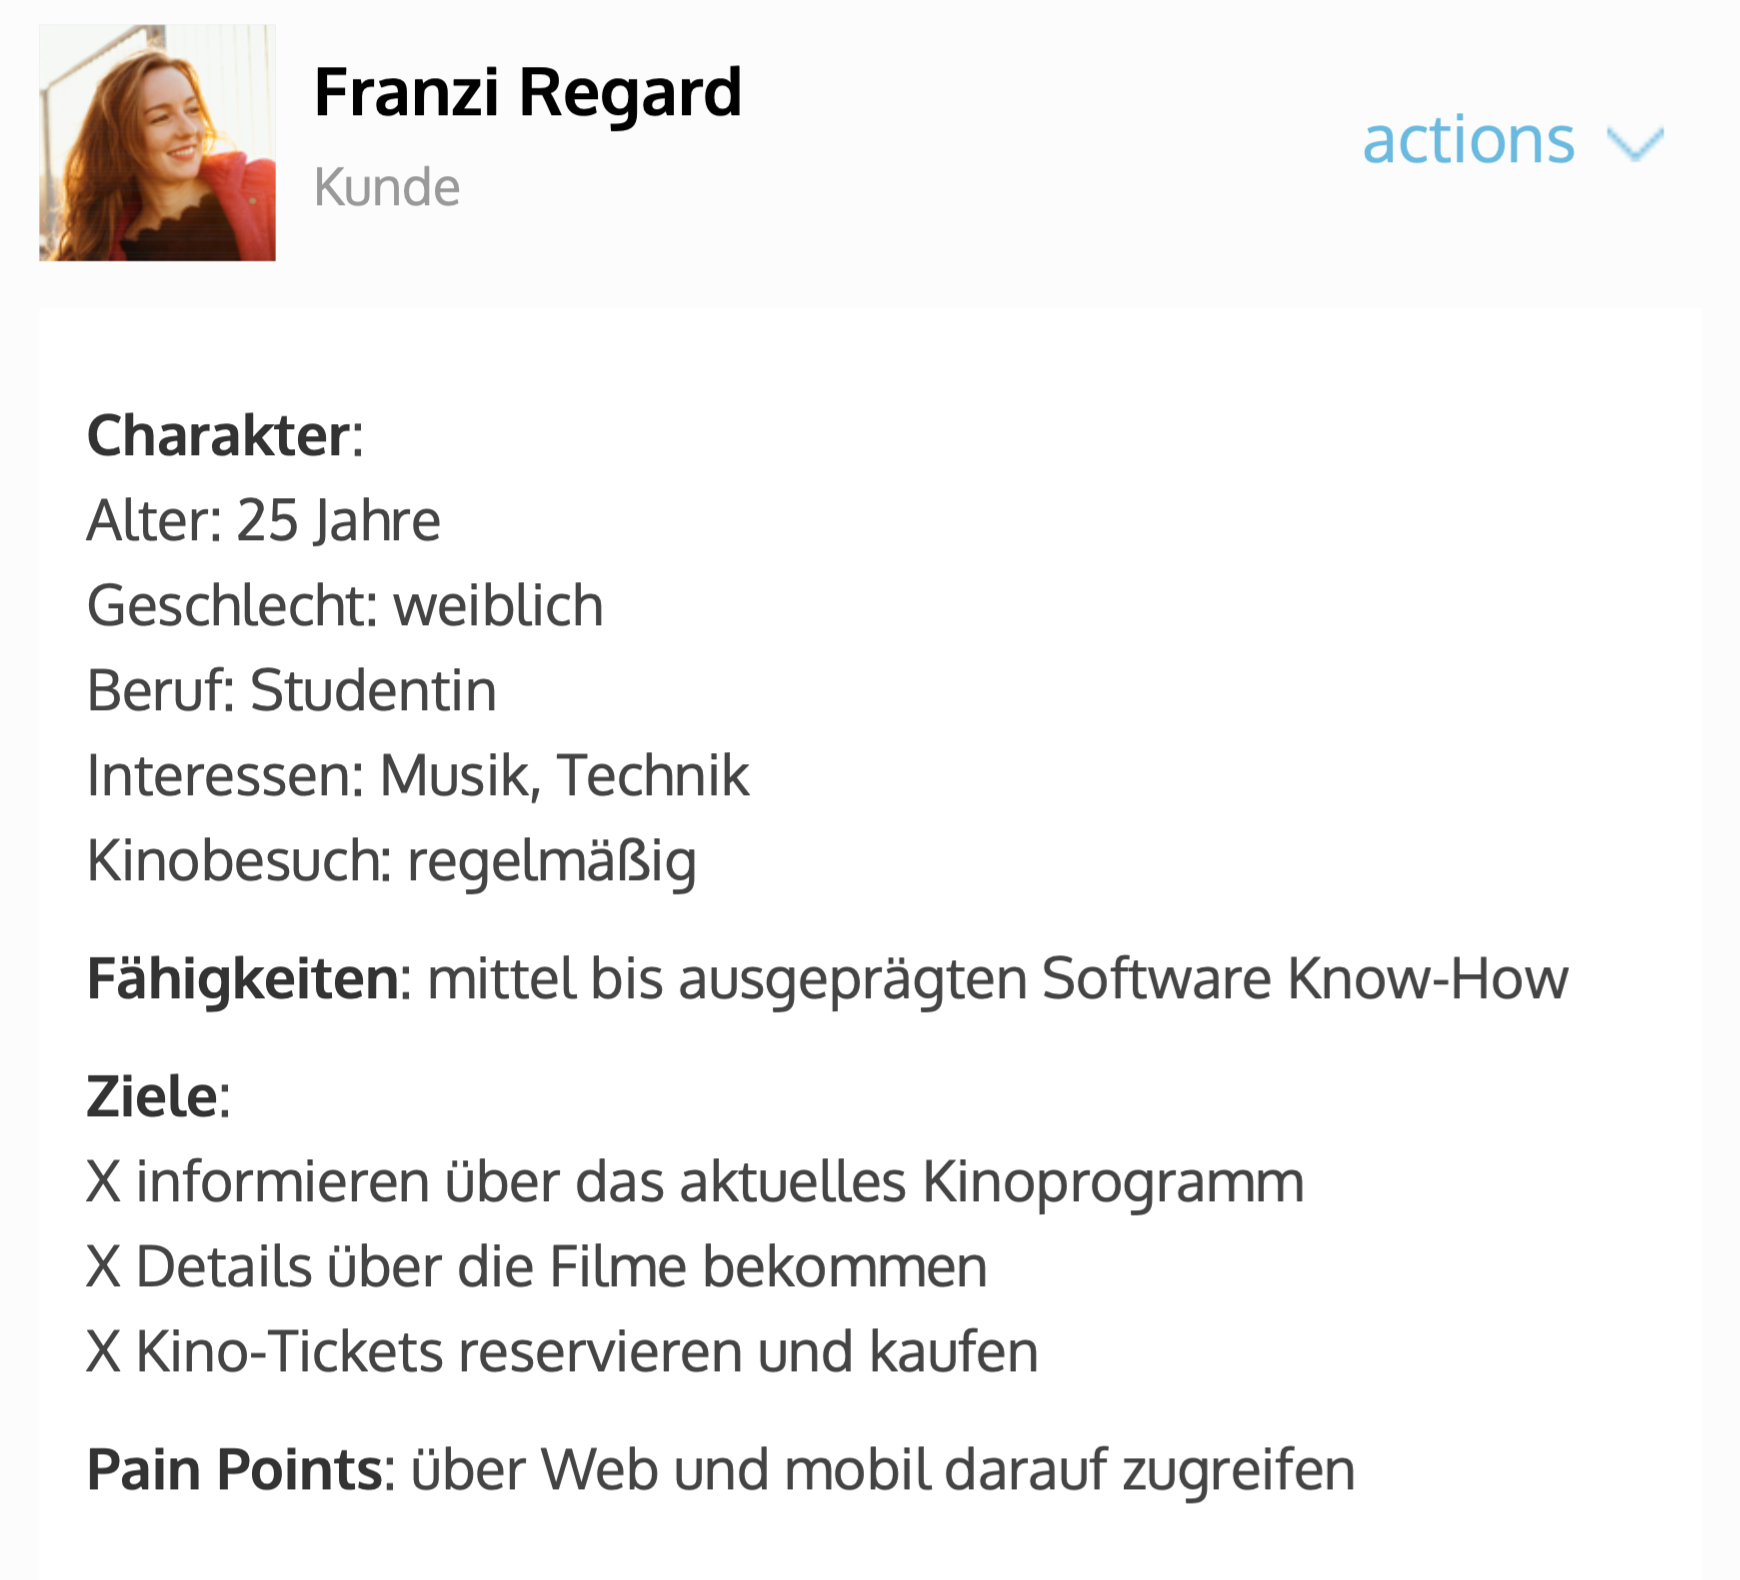
\includegraphics[width=0.49\textwidth]{img/franzi.png}} 
			\subfigure[Persona Gustav]{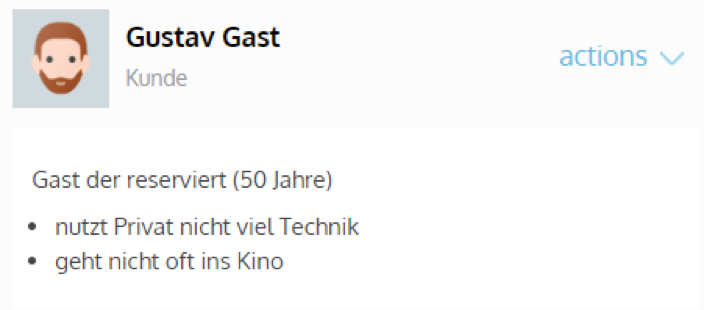
\includegraphics[width=0.49\textwidth]{img/gustav.png}} 
			\subfigure[Persona Kassandra]{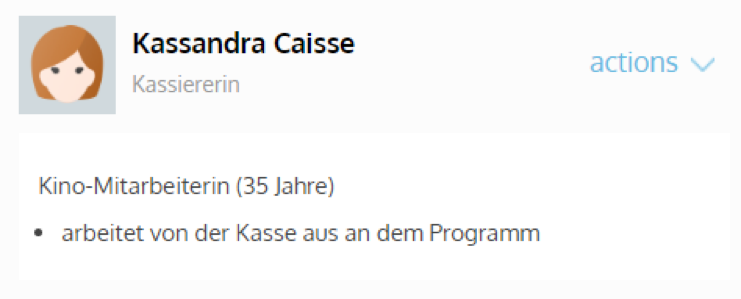
\includegraphics[width=0.49\textwidth]{img/kassandra.png}} 
			\subfigure[Persona Walter]{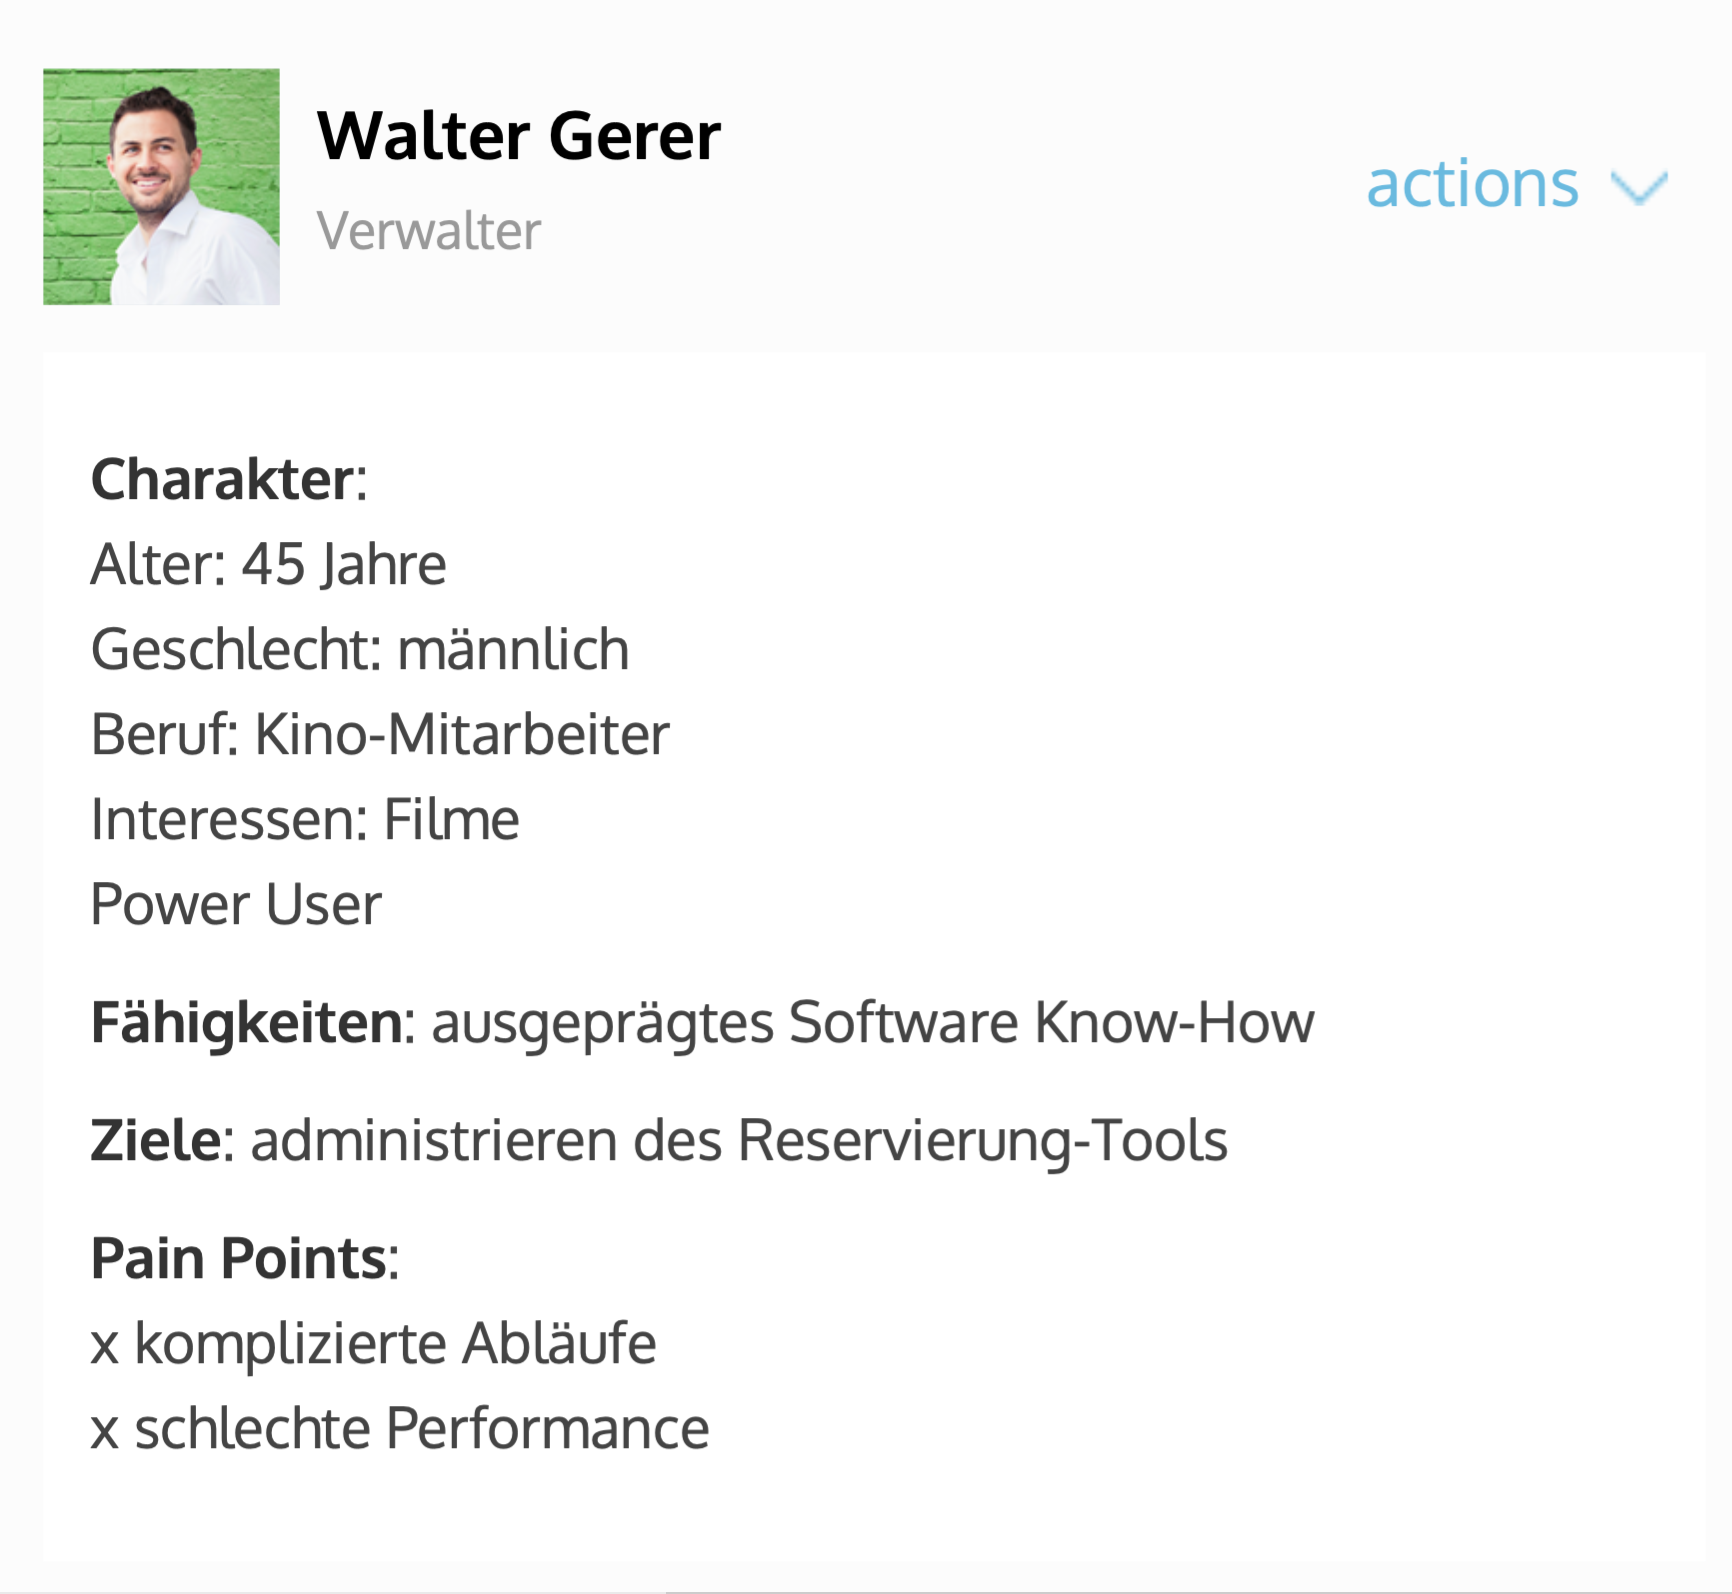
\includegraphics[width=0.49\textwidth]{img/walter.png}} 
			\caption[Personas ]{\label{fig:personas}Personas [DRAFT - detaillierter!] }
		\end{figure} 
		
		Darauf aufbauend werden Use Cases für die Personas entwickelt. Diese beschreiben Szenarien, wie die Personas das Endprodukt verwenden werden und welche Vorgehensweisen und Anforderungen dabei haben. 
		
		\begin{figure}[H]
			\begin{tabular}{p{13cm}}
				\textbf{Franzi Regard} \\\toprule
				Als Franzi möchte ich mich schnell vom meinem Smartphone oder Laptop aus über das aktuelle Kino-Programm informieren und Kino-Tickets reservieren und kaufen, um mit meinen Freunden einen Film anzuschauen. Dabei lege ich viel Wert auf ansprechendes Design und eine schnelle Abwicklung.
			\end{tabular}
			\caption[Use Case Franzi]{\label{fig:useCaseFranzi} Use Case Franzi [DRAFT]}
		\end{figure}
	
		\begin{figure}[H]
			\begin{tabular}{p{13cm}}
				\textbf{Gustav Gast} \\\toprule
				Als Gustav möchte ich Kino-Tickets reservieren, um mit meiner Familie einen Familienabend zu verbringen. Eine intuitive Anwendung ist für mich sehr wichtig, weil noch nie online Tickets reserviert habe. 
			\end{tabular}
			\caption[Use Case Gustav]{\label{fig:useCaseGustav} Use Case Gustav [DRAFT]}
		\end{figure}
	
		\begin{figure}[H]
			\begin{tabular}{p{13cm}}
				\textbf{Kassandra Caisse} \\\toprule
				Als Kassandra möchte ich mir die Reservierungen anschauen und Reservierungen anpassen können. 
			\end{tabular}
			\caption[Use Case Kassandra]{\label{fig:useCaseKassandra} Use Case Kassandra [DRAFT]}
		\end{figure}

		\begin{figure}[H]
			\begin{tabular}{p{13cm}}
				\textbf{Walter Gerer} \\\toprule
				Als Walter möchte ich das Kino-Programm verwalten und einpflegen. 
			\end{tabular}
			\caption[Use Case Walter]{\label{fig:useCaseWalter} Use Case Walter [DRAFT]}
		\end{figure}
		
		Schließlich wird aus den Personas eine User-Story-Map erstellt. In dieser werden die daraus hervorgehenden Features visuell geplant und in unterschiedliche Releases priorisiert. 
		
	\begin{center}
		{\textbf{[User-Story-Map // Größe?]}}
	\end{center}
		
	 	
%		\subsection{Vorgabe}
%		\subsection{Rahmenbedingungen}
%		\subsection{Bewertungskriterien}